\section{Tasks, Projects and Activities}
\subsection{Dairy tasks and activities}
Actually, the development of website is function-oriented, the branch "master" is the principal branch which will be released to the public, besides every one or two weeks, a new branch which means a new feature was added into the website. And also every new feature need to be tested before merging into the "master" branch.

\begin{figure}[h!]
    \centering
    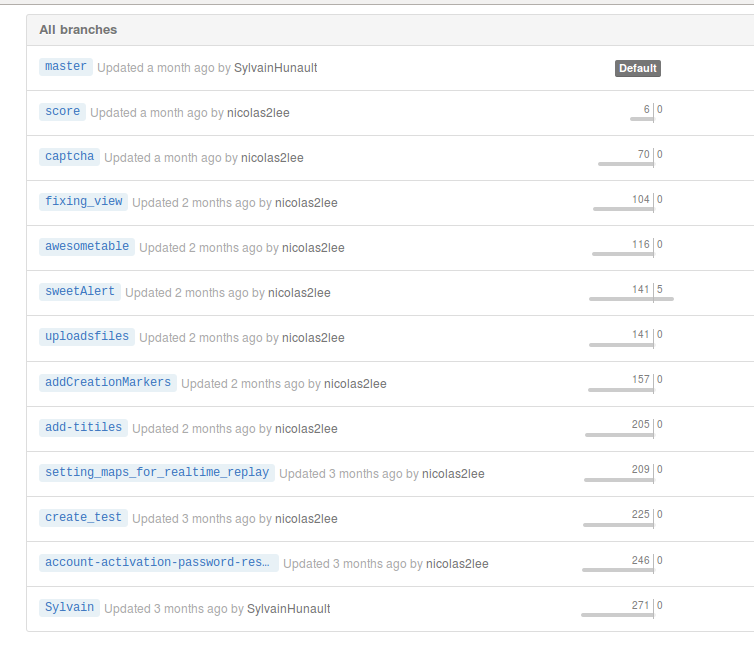
\includegraphics[width=12cm]{allbranches.png}
    \caption{All function-oriented branches }
    \label{fig-sample}
\end{figure}

%============ new features
\subsection{New features}
%============ New style and New Home Page
\subsubsection{New style and New GUI}
%\begin{figure}[h!]
%    \centering
%    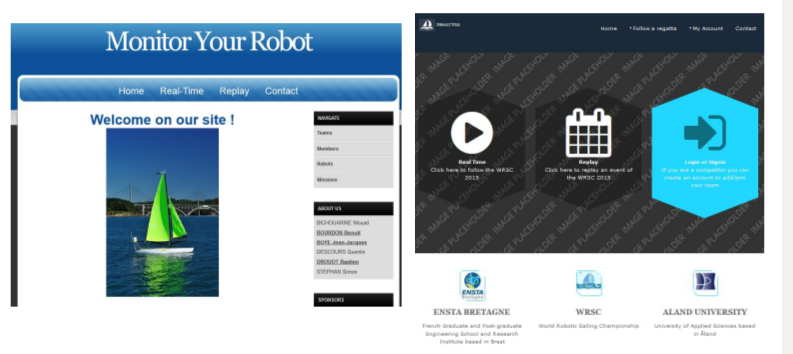
\includegraphics[width=20cm]{oldversion.png}
%    \caption{old version GUI }
%    \label{fig-sample}
%\end{figure}
\begin{figure}[h!]
\centering
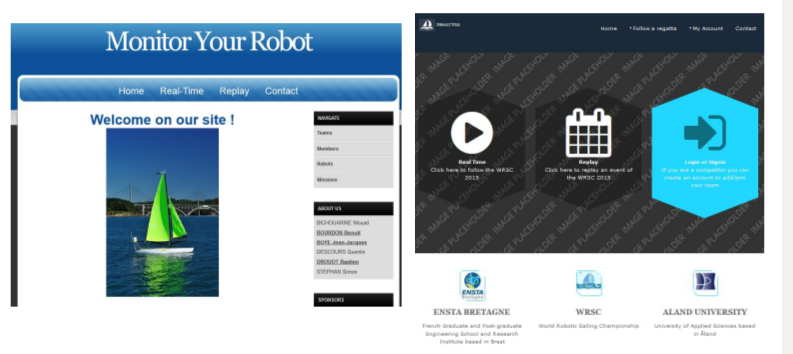
\includegraphics[width=14cm]{oldversion.png}
\caption{old home page, WRSC2014, MYR2015 }
\label{fig-sample}
\end{figure}
The web site created for the WRSC 2014 (project SWARMON) contains a no open sources CSS and Layout(left image in the figure before), and at the beginning of 2015, the web site was updated with the latest CSS3 which is open sources and more beautiful and customizable(right image in the figure before). Our current web site based on the latest CSS3.
\begin{figure}[h!]
\centering
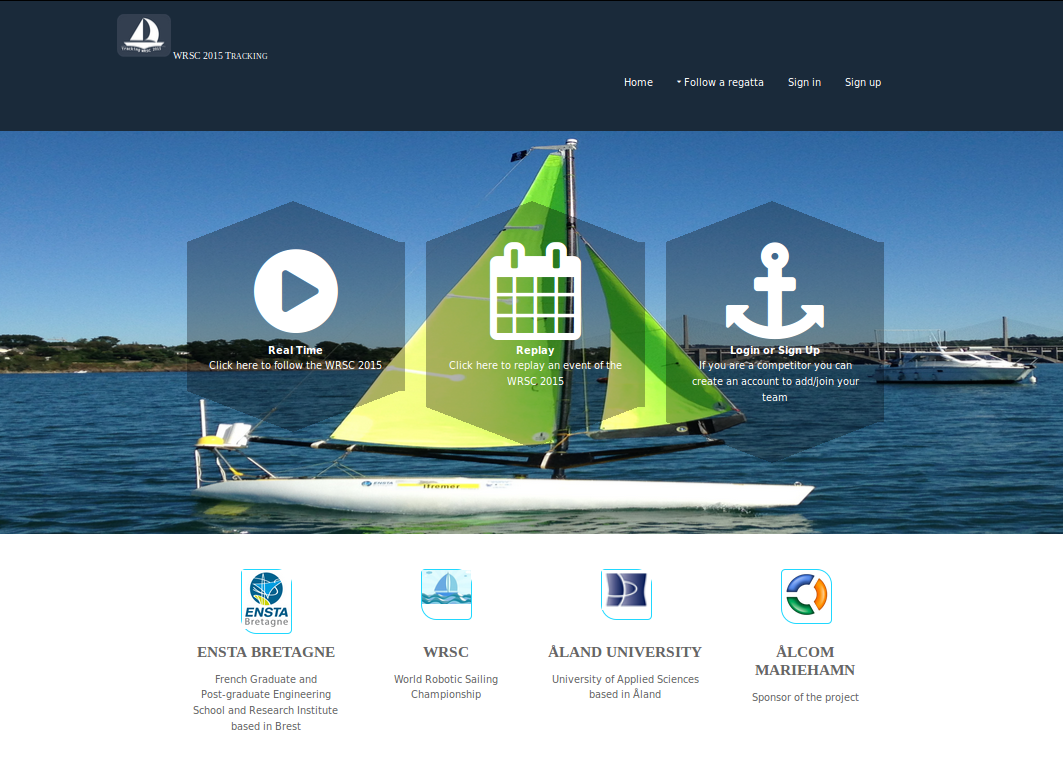
\includegraphics[width=13cm]{homepage.png}
\caption{New Home Page }
\end{figure}

%====== add team#show
\begin{figure}[h!]
\centering
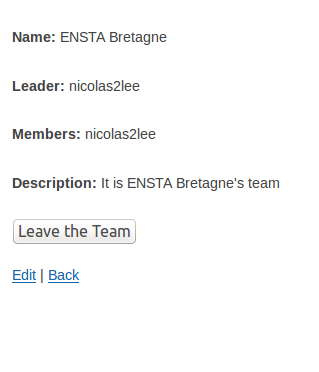
\includegraphics[width=15cm]{oldteamshow.png}
\caption{old team show}
\label{fig-sample}
\end{figure}
In the previous version, the web site could only display the basic information about every team, like: team name, leader, members and description. In order to simplify the access, we add two fields by using two Ajax requests to permit the management of members and robots, so team leader could kick their members by itself rather than ask the administrator to do so. 

%====== add robot#show
Similar to the page team\#show, the previous web site could only display the basic information about every robot, like: name, owner(team), category. These information are essential but insufficient, especially for the new visitors, the users do not know which mission their robot participated (if they want to know, they need to go to the page attempts, and check their robot name in the whole list one by one and also if they want to know the time for missions, or/and the time for every attempt, they need to go another page to check all the information). So in order to facilitate the use of web site, we decided to put all these information into the page robot\#show. Also we had thought a lot about the form to display all these information to users, since the logic is that a robot participates several missions, and for every mission, there could be more attempts, and every score and tracker id were attached to an attempt. So based on this hierarchical order, it will better to choose a tree structure chart to show the logic. In order to meet our need, we had chosen google org charts which are open sources and all APIs are provided and published by Google company. Since our web site was built up by ruby on rails, and google org charts were released as JavaScript APIs, from this, every time when the site loading the robot\#show page, it will recall a Ajax request and send all the associated information to the JavaScript part, then in the JavaScript part, we could use the org charts' APIs directly. 
\begin{figure}[h!]
\centering
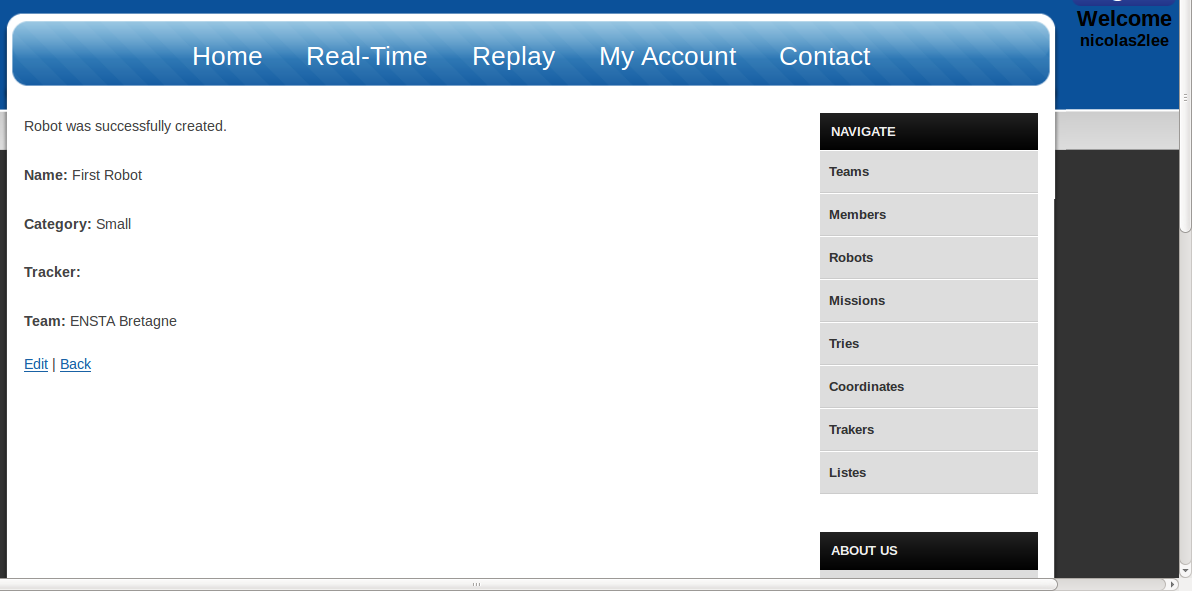
\includegraphics[width=15cm]{oldrobots.png}
\caption{old robot show}
\label{fig-sample}
\end{figure}
\begin{figure}[h!]
\centering
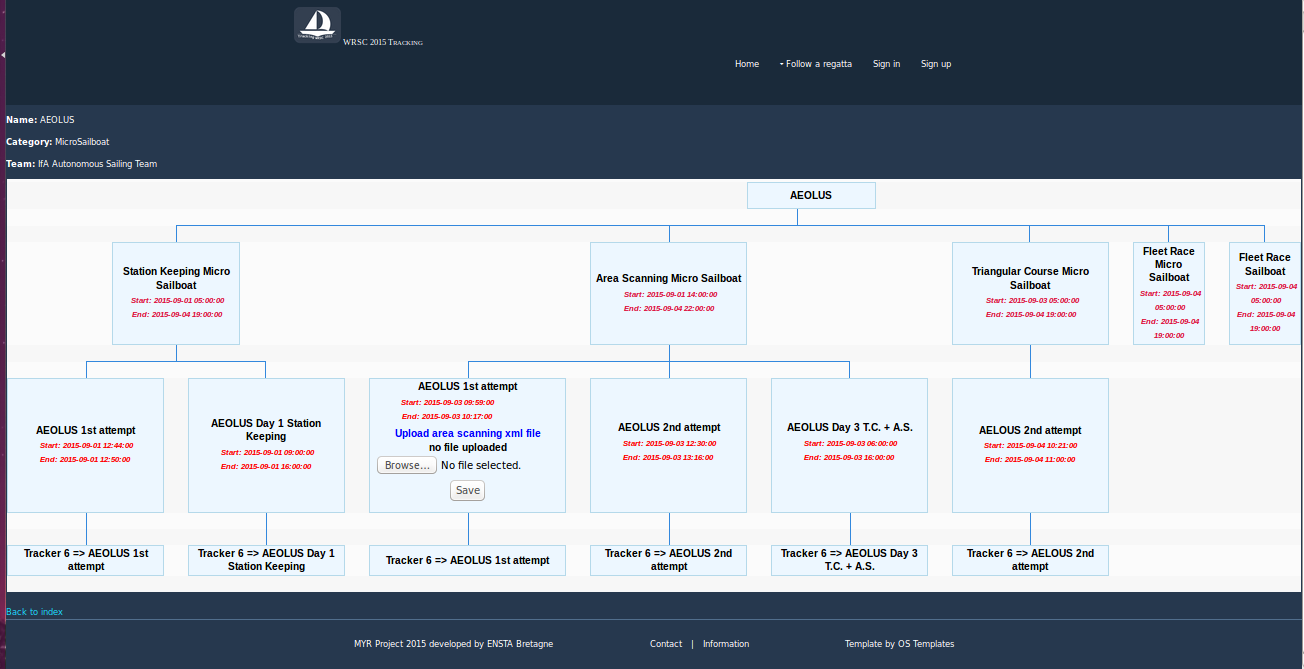
\includegraphics[width=15cm]{orgcharts.png}
\caption{Google org charts example }
\label{fig-sample}
\end{figure}

%============== Sortable \& Searchable Table
\subsubsection{Sortable \& Searchable Table}

The previous version web site(WRSC 2014 in Galway) used a table to list all the information for teams, robots, missions, members and etc. And all these tables are only sortable by the alphabetic order.
\begin{figure}[h!]
\centering
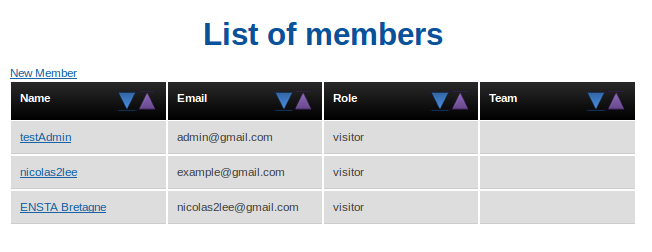
\includegraphics[width=15cm]{oldtable.png}
\caption{WRSC 2014 searchable only table }
\label{fig-sample}
\end{figure}
The only sortable table works well when there is not enormous data, if we suppose that there are more than 100 members in our database, and if you want to find the information about one member and you had only the name of this member, it will be stupid to check the whole list just by eyes. Furthermore, if the web site displays more than 10 records in one page, which often makes the user feeling uncomfortable and inefficient. Based on these reasons, we choose a flexible and customisable JavaScript plug-in "DataTable". DataTables is very simple to use as a jQuery plug-in with a huge range of customisable option, and the functions which we are interested most are sorting(which makes the table sortable by alphabetic order), filtering (which makes the table searchable, we can search one element by typing part of the keyword) and pagination (which limits the number of elements in one page, also it will make the page loading be faster and reduce the pressure of server because of the limitation of elements in the page). What's more, "DataTable" provides more APIs which also make the html table flexible, the developers are easy to get the index or element in the table just by calling the functions, comparing to the static html table, the "DataTable" is more dynamic and interacted for users.
\begin{figure}[h!]
\centering
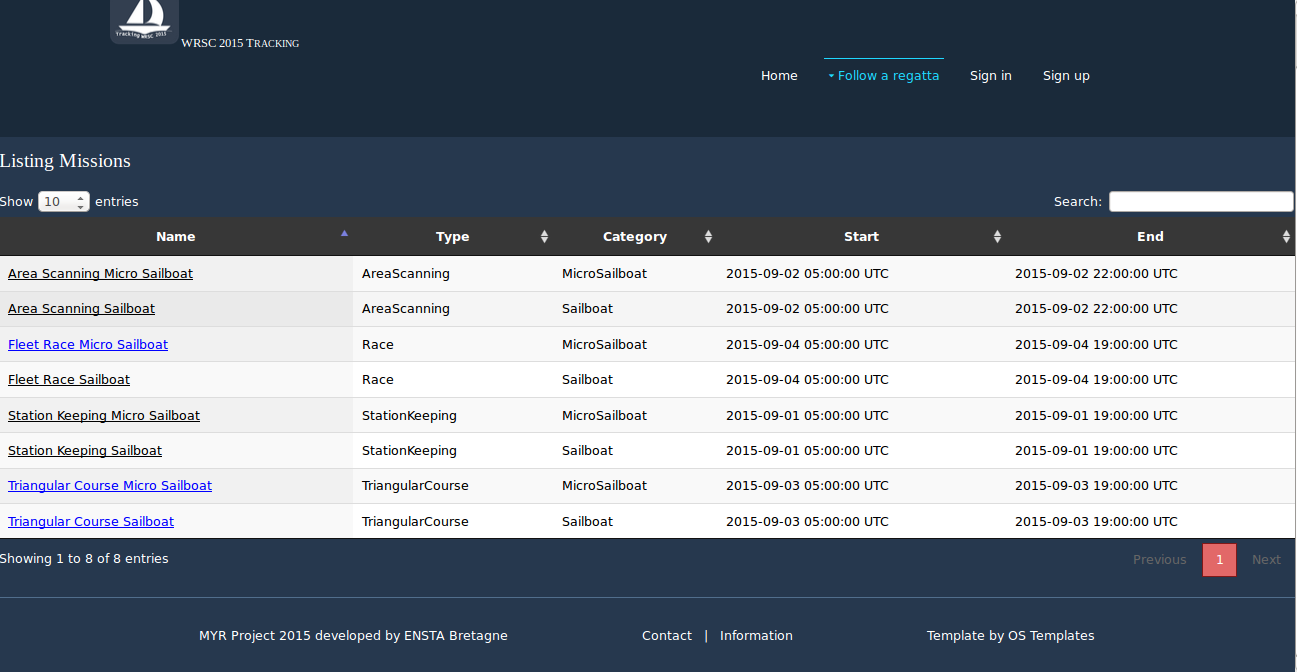
\includegraphics[width=15cm]{DataTable.png}
\caption{DataTable plug-in example }
\label{fig-sample}
\end{figure}

\subsubsection{Improved Account Management}
\begin{enumerate}
\item{Signup}
\begin{figure}[h!]
\centering
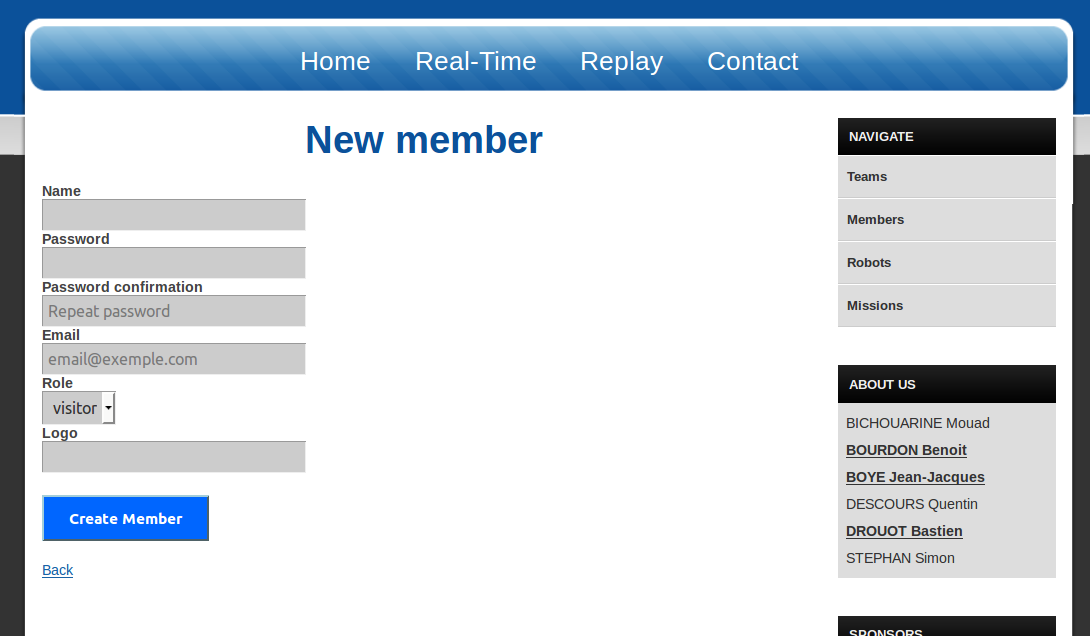
\includegraphics[width=15cm]{oldsignup.png}
\caption{old sign up }
\label{fig-sample}
\end{figure}

\begin{figure}[h!]
\centering
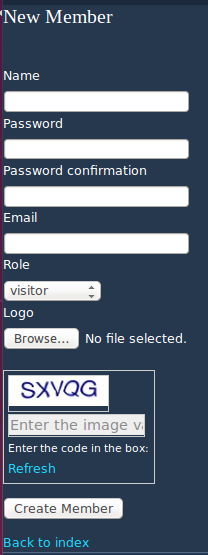
\includegraphics[width=15cm]{newsignup.png}
\caption{new sign up }
\label{fig-sample}
\end{figure}

The new sign up page add two new features:
\begin{itemize}
\item{Uploading local image file instead of typing a link}


In the old version web site, the user could only typing an image file url to upload the logo. And at the side of server, it adopts a gem called "fastimage", which could handle of the url and get the image of this url, but one limitation is the image size could not larger than several hundred pixels * several hundred pixels, as a matter of fact, this size is quite small comparing to the normal image file which is nearly several mega bytes. So for this reason, the logo field is nearly useless because of the inconvenient. 
\paragraph{Software requirements}
In the new website, we used a gem called "carrierwave"(an open sources free project, all the codes are available in their Github repertoire), which permit to upload no matter what format file. Furthermore, here we need to treat the image file, so at the side of rails application, it requires another gem "mini\_magick"(Unlike RMagick, MiniMagick is a much thinner wrapper around ImageMagick, that's why we choose MiniMagick rather than RMagick), at the side of server machine, it requires the software "ImageMagick" (under Linux, type "convert -v" to check if the "ImageMagick" was installed).
\paragraph{Apply to web site}
Once all the gems are installed successfully, a new folder "uploaders" will be added into Rails.root(the root path of rails application)/app/uploaders, and the creation of uploading action is similar to create a controller/model in rails application, either by the command "rails generate uploader nameoffile", or by create the file manually. And then in the model, we need to mount the uploader, in our case, we need to add  "mount\_uploader :logo, MemberlogoUploader" in the file Rails.root/app/models/member.rb. After that, the attribute logo of member would only accept a file uploader object, even at the beginning, we define the type of logo is a string. If we dive deep into the database(either look through by rails console, or by SQLite database browser, the attribute logo is filled by a complicated object where it contains the original file name which means the name of uploaded image file, also the name of full name which means the uploaded image file's absolute file name--path in the rails application + file name and other information). Due to this reason, once an image file was uploaded, we should not change the position of this file, because in the database, the image file was just saved as the path and the name rather than the image self.


What's more, "carrierwave" provided some other customizable convenient options, for instance, we can define our own store directory to put all the image files. Actually by default, all the files accessible for any other user should be put into Rails.root/public. But do not trust the file uploaded via internet, so we should make sure all the files in public directory were inexecutable. From this, "carrierwave" also provide an option to set the extension white list, where we can limit the file format to avoid the virus. In addition, if the rails application was launched by a Linux machine, we can set the permission of the directory public to make sure all the users except the owner(admin) could only read and write, but not execute. One way possible to do so is by using the command "chmod 766 <directory>", then with the command "ls -l", we can check if the directory permission is
"drwxrw-rw-".

Also we can define different versions of image files with different sizes based on the same image, which will be applied once the image file was uploaded.

\item{Simple captcha}
Another important change for the sign up page is that we added the captcha to filtering human user and avoid basic attacks. The realization of captcha is also simple. We used a gem called "simple\_capthca2"(an open sources free project, all the codes are also available from Github repertoire). 
As controller Based, we just need to do:
Add the following line in the file “app/controllers/application.rb”
\begin{lstlisting}
ApplicationController < ActionController::Base
  include SimpleCaptcha::ControllerHelpers
end
\end{lstlisting}

In the view file within the form tags add this code
\begin{lstlisting}
<%= show_simple_captcha %>
\end{lstlisting}

and in the controller's action authenticate it as
\begin{lstlisting}[language=Ruby]
if simple_captcha_valid?
  do this
else
  do that
end
\end{lstlisting}
\item{Activate by email}
In the new web site, also we add the function of sending emails to activate the new account when one user register on the site. As we do not have any specific email account, we choose Gmail account as our admin email account because of several reasons.
\begin{itemize}
\item In order to display the google map in our web site, we register a google account to obtain a google map JavaScript API key, so already even we did not choose Gmail as our main email, we should at least use the google account for JavaScript API.
\item Gmail service is free and easy to use, although Google limits the amount of mail a user can send, via its portable SMTP server, and the amount of sending emails is limited 99 per day, regarding our web site is focused on the participates, even maybe there are some other users, 99 is already enough for the email function. In addition, if we want much more capacity, if the budget allows, we could buy the service of Gmail SMTP server in the future.
\item Gmail is secure, wide used and compatible with others email service provider. And sometimes, Gmail is too secure to use. And the problem we meet at the beginning is that we had sent an email by configuring the SMTP server in our Rails Application, then Google detected this operation was done by machine not a web user and our email was blocked. In order to solve these types of problems, we need to configure our Gmail to less secure status by going to this page https://www.google.com/settings/security/lesssecureapps and changing to less secure.
\end{itemize}
When the Gmail account was setted correctly, and also we can send emails to other users, another problem came to our views. How can we send a unique link to the user and also how can we identify this link is associated with the relative user ? Actually before create a user, we create a new activate token(which is used to send to the user) and a activate digest(which is saved into database and used to identify the relative user). 
In the file Rails.root/app/models/member.rb
\begin{lstlisting}
	before_create :create_activation_digest
	def create_activation_digest
		self.activation_token  = Member.new_token
		self.activation_digest = Member.digest(activation_token)
	end
\end{lstlisting}
In fact, all the passwords, or more generally, the important information are encrypted before saving into the database by using the popular gem "Bcrypt". Obviously the security of encryption depends on the longer of generated token(Here we used 64 bits to generate a random token, normally it is long enough) and the algorithm(In this case, it is "Eksblowfish"--"expensive key schedule Blowfish", which based on the algorithm Blowfish. Cryptotheoretically, this is no stronger than the standard Blowfish key schedule). Also we need to pass the user's email address as an argument in the url, then we can identify the token with the member which was saved in the database found by the email address.
In the file Rails.root/app/models/member.rb
\begin{lstlisting}
    def Member.digest(string)
   		cost = ActiveModel::SecurePassword.min_cost ? 
   			   BCrypt::Engine::MIN_COST : BCrypt::Engine.cost
		BCrypt::Password.create(string, cost: cost)
    end
    
    def Member.new_token
   	 	SecureRandom.urlsafe_base64
   	end
\end{lstlisting}
Then the creation of email sending is just like any other page, firstly create the controller with desired actions, and then create the views which would be sent to the user later.
\end{itemize}

\item{Sign in}

In the new sign in page, we had also added two new features:
\begin{itemize}
\item{Remember the User}
The function of "Remember me" is quite similar to sending the activation link to users. If the user choose to remember in the computer, then the server would write the user id and a remember token into cookies, with the function cookies.signed which provided by rails application, the contents in the cookies would be encrypted. Furthermore, something should be noticed: 
\begin{itemize}
\item Cookies exist in different browsers in the same computer, so if the user has more than one browser (for instance: one Firefox and one Chrome), the cookies will be shared between the two browsers. 
\item The contents in the cookies contains two values, one is what we want to save into the cookie, and the other one is the expire date which indicates the validate time for cookie. If we use "session", which contains the same contents as cookies, but the expire date is from when the contents were created to when the user close the browser.
\end{itemize} 

\item{Reset the Password}
"Reset the password" has the similar principle as the activation email sending. When a user request to reset its password, it needs to provide its email address as a reference. Then the server generate a token and a digest, send the link which contains the user's email address and a reset token to the user. After, when the user clicked the link, the server verifies the digest with the token, if it is the correct token, then the user could change its information.
\end{itemize}
\begin{figure}[h!]
\centering
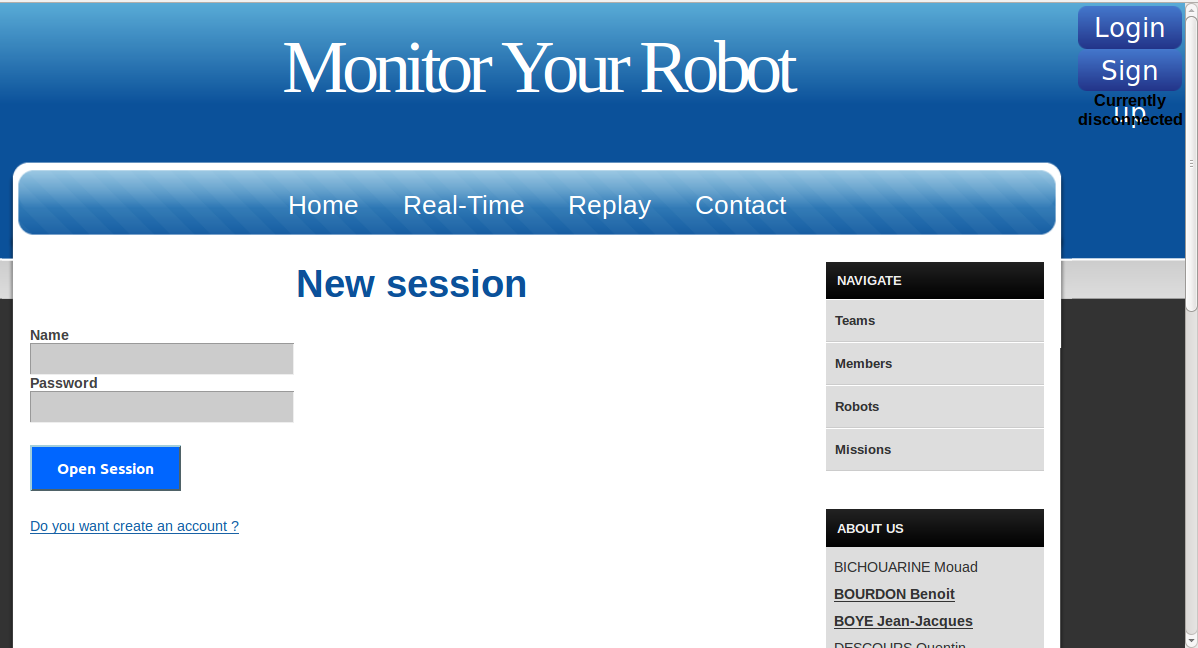
\includegraphics[width=15cm]{oldsignin.png}
\caption{old sign in }
\label{fig-sample}
\end{figure}

\begin{figure}[h!]
\centering
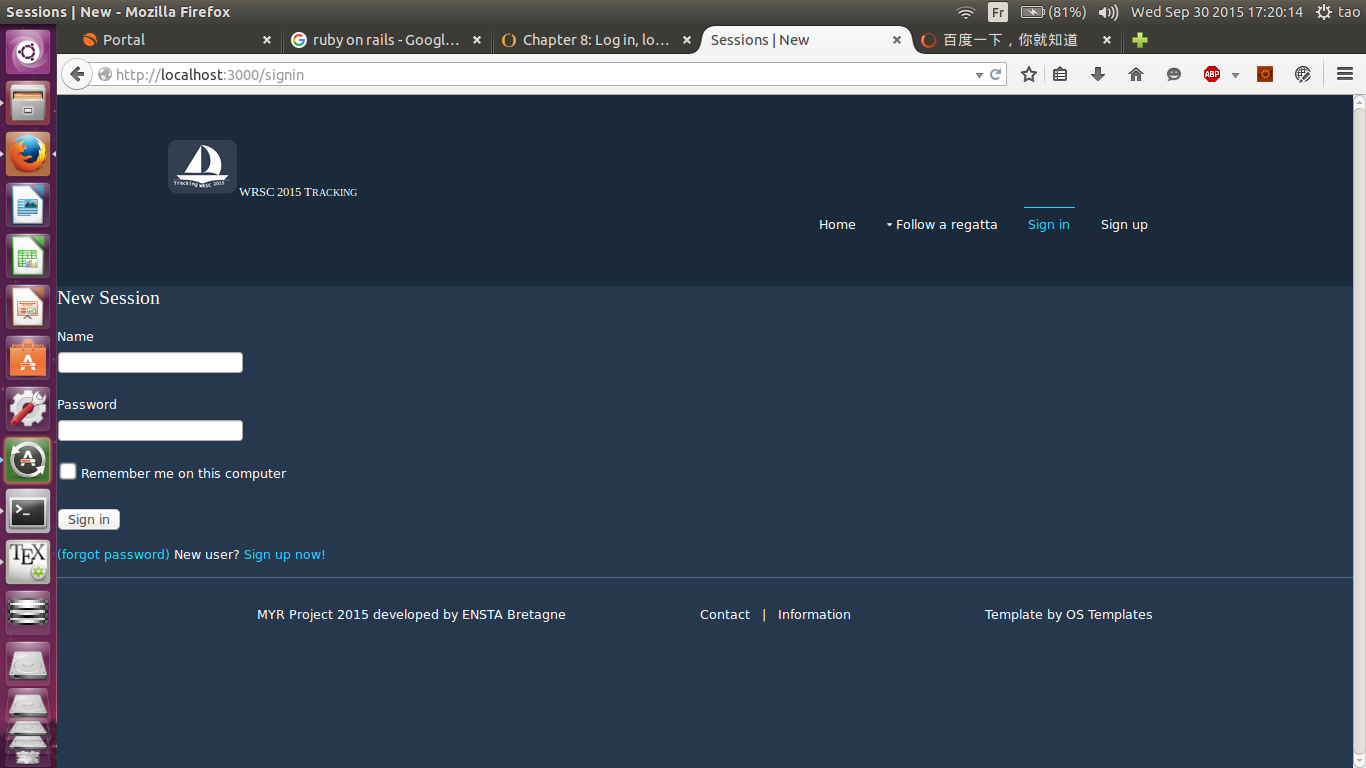
\includegraphics[width=15cm]{newsignin.png}
\caption{new sign in }
\label{fig-sample}
\end{figure}


\end{enumerate}


